\label{adaptive_cooperation}
Adaptive traffic control systems aims to coordinate signal controlled intersections so as to optimize some performance index eg. average delay or number of stops (or a combination) but also to reduce the need for constant supervision and tuning of intersections.

They do this by dynamically adjusting cycle times, phase sequences and green splits according to detected as well as predicted traffic and thereby reacting to those dynamic aspects of traffic, which cannot be captured by the static optimization routines used to generate time-of-day plans. Some authors (\cite{1}, \cite{44}, \cite{46}, \cite{scoot2004}) even skip or work around the conventional periodic scheme based on a common cycle time and make direct assignments of phases and allow phases to be skipped, as presented in section \ref{dynamicmodel}. 

It is evident that the cycle time is crucial in optimization because, for a congested network, increasing the cycle time will always cause a throughput increase (there are always cars waiting to cross the intersection). In the litterature the cycle time is often common to all intersections under traffic control so that green waves (arterial progression) can be produced. For direct assignment systems the throughput is dependent on allocation to phases of consecutive green time. Long cycle times lead to long phase durations, which allow a steady flow of vehicles to pass and minimizes lost and interphase time per time unit.

For large networks the enforcement of a common cycle time is inappropriate, however. Consider a network which is so large that two disjoint arterials exist. In this case it is unlikely that a common cycle time will allow green waves to exist for both arterials eg. when the intersections of one arterial are more tightly spaced than in the other. For networks of this type (size) a direct phase assignment model might provide the necessary flexibility. Even though the arterials cannot be considered as a single arterial, they are not completely disjoint due to the effects of chaos theory. Otherwise it would make no sense to control the intersections in the area as  a single network.

Another feature of considering very large networks is the possibility of traffic redirection. If it is detected - or predicted - that an arterial is, or will be, congested under current flow conditions it is sensible to redirect some traffic onto alternative routes. 
Redirecting traffic using traffic signals is a subtle technique which has not received much research yet, though it could pose more efficient than current traffic information systems, which inform road users of congestions and alternative routes, but allows them to ignore the advice.

In this section some in-depth discussions are given for three adaptive systems, which do not rely on offline optimization as it was sketched in section \ref{offline}. The systems are:

\begin{enumerate}
\item \textbf{RHODES} by Pitu Mirchandani and Larry Head presented in \cite{44} - a hierarchical system for network-wide optimization
\item A \textbf{Phase-by-Phase} optimization strategy by Michael Shenoda and Randy Machemehl presented in \cite{1} - a system using the metaheuristic tabu search for determining greens for isolated intersections in a phase-by-phase manner
\item \textbf{DOGS} by Danish Technical Traffic Solution (TTS) evaluated in the danish article \cite{dogs}, which provides criteria-based capacity increases along an arterial
\end{enumerate}

Comparisons will be made for the systems to highlight differences in areas such as \textit{detection}, \textit{prediction} and \textit{optimization strategy}.

\subsection{RHODES}
\label{sec:rhodes}

RHODES approach to traffic signal optimization is a hierarchical one
with 3 layers of detail, see Figure \ref{fig:rhodes_hierarchi}.

The macroscopic layer performs \textit{dynamic network loading}, which
involves observing changes in the aggregated flow data of the entire
network due to variations in the OD matrices. This layer supplies
estimates of link flows to the middle level in rough numbers
eg. vehicles per hour.

The mesoscopic middle layer considers sectors of the network eg. an
arterial. This \textit{network flow control} layer work in the detail
level of platoons and average speeds. Green time is allocated to
phases to accommodate the movements of the platoons and so
coordination of intersections is done at this level.

At the lowest level is \textit{intersection control} where vehicles
are handled individually (a microscopic layer). Here the green times
and phase ordering suggested by the middle layer are fine tuned.

\begin{figure}[!ht]
\begin{center}
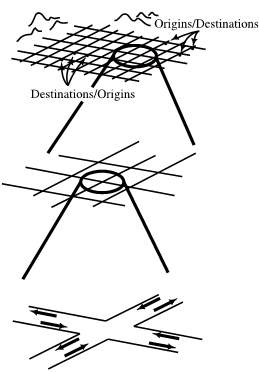
\includegraphics[scale=0.5]{rhodes_hierachy.png} 
\end{center}
\caption{The three levels of detail: network, sector, and intersection}
\label{fig:rhodes_hierarchi}
\end{figure}

An adaptive traffic control system must operate quickly in order to
adapt signals to traffic in real-time. The RHODES platform has good
decomposition opportunities and is pluggable ie. the upper level is a
black box feeding the lower level with predictions and
optimizations. At the time the article was written, the top level of
RHODES had not received much development and thus only the middle and
lower level are described herein.

\subsubsection*{Detection}
Detection methods are not discussed in detail in the paper. They can
be of any technology including induction loops and video.

\begin{figure}[!ht]
\begin{center}
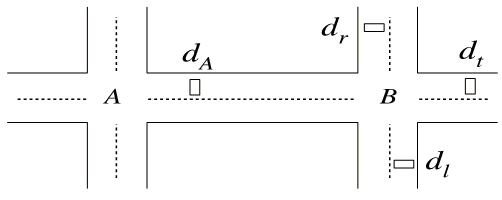
\includegraphics[scale=0.5]{rhodes_prediction-strategy.png} 
\end{center}
\caption{Detector placement and propagation of information in a simple grid}
\label{fig:rhodes_predict}
\end{figure}

\subsubsection*{Prediction}
The PREDICT method by the co-author, XXX Head 1995 XXX, is used to make
predictions for individual vehicles. PREDICT is built for network
prediction and relies on the fact that incoming flow to an
intersection originates from adjacent intersections. This concept can
be explained from Figure \ref{fig:rhodes_predict} where traffic
detected at $d_a$ is the sum of right-turning traffic at detector
$d_r$, left turning traffic at $d_l$ and through-going traffic at
$d_t$.

Thus given flow estimates for the links facing intersection B and
turning probabilities for each link an estimate can be given for the
inflow to intersection A from east. On the link between the two
intersections there will be traffic entering and exiting the system,
but these contributions - and losses - to the traffic, which can be
measured at $d_a$, are expected to be very small.

Prediction of arrival times of the vehicles which has passed detectors
$d_{\lbrace r,t,l \rbrace}$ depend on the current phase at
intersection B and queue conditions. Mirchandani and Head has
identified four cases, which cover arrivals to an intersection, which
are summarized in table \ref{tbl:delaycases}.

\begin{table}[!ht]
\begin{center}
\begin{tabular}{l|ll}
 & \textbf{Green} & \textbf{Red} \\ \hline
\textbf{No queue} & 0 & $T_G$ \\
\textbf{Queue} & $T_Q$ & $T_G$ + $T_Q$
\end{tabular}
\end{center}
\caption{Delay incurred for a vehicle arriving to an intersection in various states where $T_Q$ is the time for ahead queue to clear and $T_G$ is the time to the next green.}
\label{tbl:delaycases}
\end{table}

In the cases involving queue there is, of course, a possibility that
the vehicle will not be able to cross the intersection before several
green phases have occurred. This is likely to happen under high
congestion when intersections are placed closely.

At the mesoscopic level, network flow control, the APRES-NET
prediction method is used. It is based on simulation and has
similarities to PREDICT, though it works in the detail level of
platoons and encompasses several intersections, not just the upstream
ones but also those upstream of the upstream intersections and so
on. Since the 2nd level must deliver complete suggestions for timing
plans for each intersection (to be fine tuned by intersection control)
it must run quickly. Performance is dependent on the number of
intersections in the monitored sector and sector sizes can thus be
scaled to match the speed requirements depending on hardware.

The prediction horizon for network flow control is 200-300
seconds. Cycle times for simple intersections with just a couple of
phases vary between 60 and 150 seconds so this horizon is plenty to
predict and respond to most types of fluctuations by performing phase
skipping, phase reordering and assignment of phase durations. The
intersection level control operates with a prediction horizon of 20-40
seconds and thus can only make decisions on whether to lengthen or
decrease the green time of phases within that horizon.

\subsubsection*{Optimization}
As in the dynamic model of section \ref{sec:dynamicmodel} timing plans are
described by phase ordering and duration independent of cycle time,
splits and offsets.  Optimization is performed on each level using
prediction results for that level.

At the network flow control level the REALBAND algorithm forms
progression bands (ie. \textit{green waves}) for platoons traversing
the sector based on the predictions from APRES-NET. This is done by
finding \textit{conflicts} between platoons, which will request access
for conflicting phases at the same time. In this way a conflict can be
regarded as the denial of green to a platoon due to the passage of
another platoon. A decision tree within the optimization horizon of
200-300 seconds is build and explored to find the configuration with
the fewest conflicts. This results in a set of phase orderings and
green times for each intersection.

At the lower level a dynamic programming approach, COP, takes the
results from REALBAND and distributes green time for some horizon to
the phases received from the above level. The phases and their
ordering must be respected so as to not introduce conflicts, which
have been resolved by REALBAND. For the same reason there are
restrictions for the maximum change in either direction of the given
green times, but COP is allowed to use its more detailed predictions
to perform the mentioned fine-tuning of green times.

\subsubsection*{Evaluation}
RHODES has been implemented and evaluated in CORSIM as part of the
evaluation for Federal Highway Administration (FHWA) inclusion in
RT-TRACS. RT-TRACS is an effort to choose and standardize a peak
performance traffic signal optimization system for American traffic
networks.

The simulation is done for an arterial of 9 intersections with steady
increase and then decrease of traffic over a 2 hour period. This is a
FHWA test case and the baseline traffic control system is
semi-actuated control based on the results of offline tools including
TRANSYT and PASSER, which represents the best-can-do from an offline
approach and can be considered a hard competitor.

Testing shows that RHODES is more capable of exploiting the capacity
of the arterial. As long as there is no congestion the throughput will
match the demand and in the comparison RHODES can simply take more
load before experiencing congestion.

Real adaptive systems should excel in the case of low demand, since
the overcapacity will then allow RHODES to, roughly said, cater for
each vehicle. The effect, compared to the semi-actuated control, is
convincing with 50\% reduction in delays for low demand and 30\%
reduction for high demand. This effect is expected to disappear when
demand reaches the capacity of the arterial in which case, for both
systems in the comparison, only throughput can be improved by
increasing the green time along the arterial and maintaining proper
coordination.

The simulation was run multiple times and for both throughput and
delay it is clear that RHODES is more consistent than semi-actuated
control and offers less variability from run to run.


\subsection{Phase-by-Phase}
The phase-by-phase (PP) system was developed to overcome a number of deficiencies, which seemed widespread in adaptive systems:

\begin{itemize}
\item Fixed cycle length and/or fixed step for variation of cycle length
\item Utilization of aggregated demand data only
\item Fixed coordination of signals along an arterial og through a network
\end{itemize}

The proposed overall scheme to improve upon these issues are the isolated optimization of intersections and more fine-grained tracking of vehicles.

The optimization process has been made independent from determination of the network state ie. detection and prediction and as such some of these subjects are mostly discussions and proposals for improvements.

\subsubsection*{Detection}
PP relies on individual tracking of vehicles to obtain an arrival based model. For networks this can be realized only with video detection with eg. license plate recognition; traditional loop detections cannot yet identify individual vehicles.

The PP system currently works for isolated intersections and so detection loops are sufficient to estimate arrival times. For detector placement, the authors suggest using simulation.

\subsubsection*{Prediction}
In the proposed form the PP system uses a Poisson process to generate interarrival times.
Alternatives are some form of time-series analysis or a Poisson process with variable mean. The use of detections made upstream could also be used, such as it is in RHODES.

The performance of PP is highly dependent on the ability of the chosen prediction system to generate proper forecasts but, as will be seen in the test results, the potential benefits are great.

\subsubsection*{Optimization}
The optimization procedure of PP seeks to minimize the stopped delay using input from the prediction process. The most widely used measure of effectiveness is stopped delay (see eg. \cite{9}, \cite{38} and \cite{31}) but the authors show that there is also a linear relationship to total travel time.

The following notation is used in the paper:

\begin{table}[!ht]
\begin{center}
\begin{tabular}{ll}
\hline
$H$ & Horizon of optimization \\
$cs$ & Cycle start time \\
$ce = cs+H$ & Cycle end time \\
$i = 1,...,N$ & Approach indexes \\
$k = 1,...,M$ & Phase indexes \\
$\lambda_k$ &  Is a partitioning of $H$ into phases and $0 = \lambda_{0} <  \lambda_{k-1} \leq \lambda_k \leq 1$ \\
$\lambda_{k_i}$ & The time into $H$ before the phase $k$, involving approach $i$, ends \\
$j$ & Vehicle id for predicted vehicle arrival within the horizon  \\
$t_{ij}$ & The arrival time for vehicle $j$ on approach $i$
\\ \hline
\end{tabular}
\end{center}
\caption{Notation}
\end{table}

$H$ should be in the order of the desired cycle time and $\lambda_k$ give the green splits and thus we have a full plan for the signal. Stopped delay can be calculated from this plan and the predicted arrivals. In Figure \ref{fig:pp_delay} this idea is sketched.

\begin{figure}[!ht]
\begin{center}
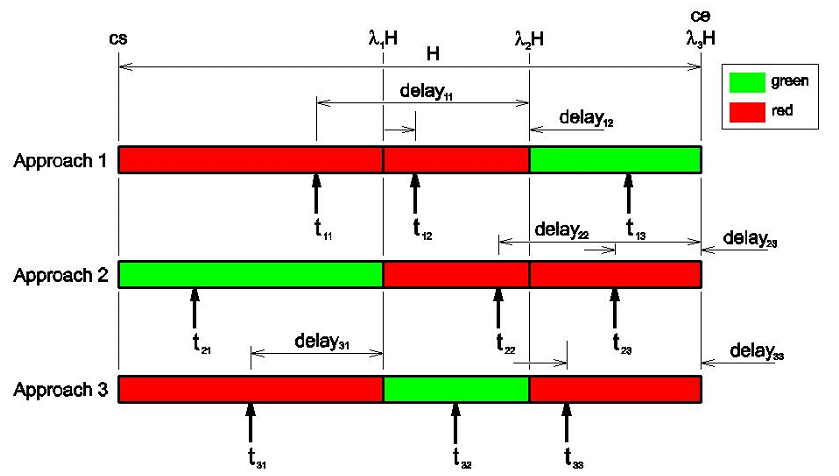
\includegraphics[scale=0.5]{phase-by-phase_delay-model.png} 
\end{center}
\caption{Calculation of stopped delay in the Phase-by-Phase system for an intersection with 3 approaches and 1 exit (no turning movements).}
\label{fig:pp_delay}
\end{figure}

In equation \ref{eqn:pp_delay} the rules for stopped delay are extracted when vehicle $j$ arrives on approach $i$ at $t_{ij}$.

\begin{equation}
delay = 
\begin{cases}
cs + H \cdot \lambda_{k_i-1} - t_{ij} & when \; t_{ij} \leq cs + H \cdot \lambda_{k_i-1} \; (before\;green)  \\
cs + H - t_{ij} & when \; t_{ij} \geq cs + H \cdot \lambda_{k_i} \; (after\;green)  \\
0 & otherwise
\end{cases}
\label{eqn:pp_delay}
\end{equation}

In the second case of equation \ref{eqn:pp_delay} vehicles incur stopped delay since they arrive after their approach has been served green time in the planning horizon. Thus they will not be served before the next green, which has not yet been planned, and stopped delay is accumulated until then. This is called carryover since vehicles are carried over into the next cycle.

PP also takes into account queue startup delay and thus cover the most critical sources of delay. However PP makes the assumption that the granting of green time to a phase will cause the approaches to be cleared completely ie. no vehicles must experience more than one green phase before they can leave.

The objective function is defined using these delay terms and thus optimization can be done by making changes in the $\lambda_k$-values within some critical points in horizon. Looking at Figure \ref{fig:pp_delay} it is seen that approach 2 is served green time until $\lambda_1 H$, supressing green from approach 1 and 3, which both have arrivals. By switching phase immediately after $t_{21}$ (setting $\lambda_1 = (t_{21} - cs)/H$) approach 1 could receive green until immediately after $t_{12}$ and so on. This example involves switching of the phase order, which was turned off in the paper.

In the PP paper \cite{1} a solution method using the above scheme is presented as a combinatorial problem. But the number of combinations increase exponentially with the number of arrivals and the number of phases. Therefore a tabu search is employed. Websters formula for optimum green time splits is used in the Proportional Heuristic to obtain a good initial solution and a 1-bit neighborhood function is defined by making changes to a single value in $\lambda_k$ (a low influence move), preserving the phase order. Candidates for the step of these changes range from the transmission time of an electronic signal ($\approx 10^{-3}s$) to the minimum headway between two vehicles travelling in a platoon ($\approx 2s$ cf. Greenshields et al. 1947).
A high influence move, which reorders phases, is also described but is turned off, as mentioned.

\subsubsection*{Evaluation}
Shenoda and Machemel compares the results of their metaheuristic search to pretimed and actuated signal control settings obtained from the CORSIM microsimulator using the test intersection in Figure \ref{fig:pp_intersection}.

\begin{figure}[!ht]
\begin{center}
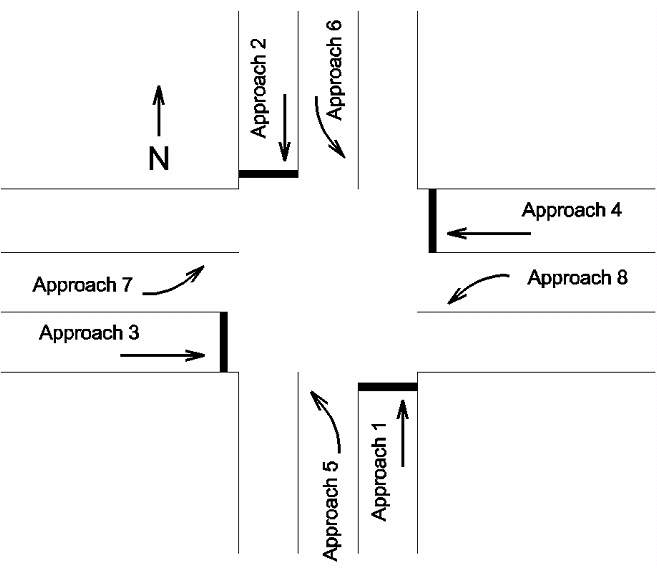
\includegraphics[scale=0.5]{phase-by-phase_testing-intersection.png} 
\end{center}
\caption{4-phase intersection from experiment \#2}
\label{fig:pp_intersection}
\end{figure}

The intersection was subjected to 8 different data sets of arrival times. In Figure \ref{fig:pp_improvements} the stopped delays for the PP system is compared to the simulation results using pretimed plans and standard traffic actuated control.

\begin{figure}[!ht]
\begin{center}
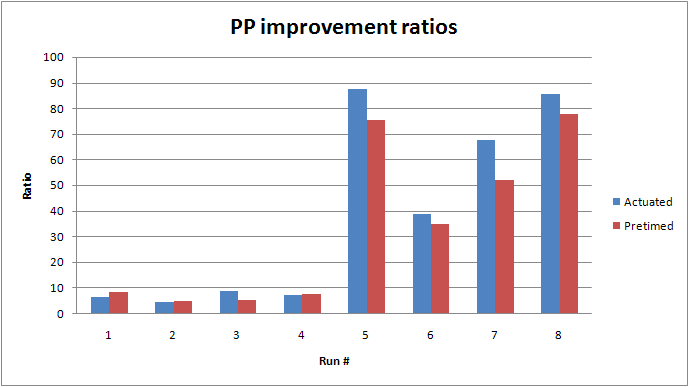
\includegraphics[scale=0.5]{phase-by-phase_improvement_ratios.png} 
\end{center}
\caption{Improvement factors of PP compared to pretimed and actuated control in the 4-phase intersection of Figure \ref{fig:pp_intersection}}
\label{fig:pp_improvements}
\end{figure}

The results should only be taken as indications since a number of assumptions were made for PP that the prediction algorithm supplied perfect information. In addition the actuated control was only semi-actuated since detectors were only used in one direction, the other being timed as in the pretimed case, which was optimized using Websters formulas.

In spite of these issues it is interesting to observe the the (semi-)actuated control strategy is not always superior to pretimed plans. It is clear, however, that both strategies are outperformed by PP. Under the given assumptions - in particular that concerning accuracy of predictions - PP can be used to establish a baseline for the best possible performance. This becomes even more true when the phase ordering constraint is dropped allowing reordering and skipping of phases.

Unfortunately Shenoda and Machemehl do not test PP on a network or even along an arterial. The optimization procedure does not consider coordination in itself though it is proposed that the prediction routine should consider departures from adjacent intersections, such as the method by Head employed in RHODES. It is speculated that such propagation of departure information could give rise to some coordination, depending on the horizon of optimization.

\subsection{DOGS}
\label{sec:dogs}

DOGS is an extension of the DOG system. The first 3 letters can be
directly translated from danish to \textit{dynamic optimization of
greens} and the appended S of the herein regarded system means
\textit{coordination}. Thus DOG is an traffic actuated optimizer for
single intersections, as described in section \ref{insec:actuated},
and DOGS add coordination. The DRD has implemented DOGS along several
arterials in Denmark.

DOGS is a criteria-based system which relies on a common cycle time
for coordination. The intended area of application is traffic signals
along arterials, which see a high fluctuation in demand.

The purpose of DOGS is to increase the capacity of the arterial in
high demand periods and revert to offline-optimized, pretimed plans in
low traffic situations. The capacity increase is realized by
increasing the common cycle time and allocate the extra green time per
cycle to the phases along the arterial. This will cause increased
delays for the minor roads, but may prevent queues from reaching the
previous intersection - or even prevent queues in cases of light
congestion.  DOGS is also capable of providing priority to buses by
extending the green time when buses are near an intersection.

At present the system must be tailored to the environment in which it
operates. For this reason the following sections will use the Herlev
area in Denmark as a reference area in order to explain certain
concepts. In Figure \ref{fig:dogs_herlev} is a layout of this network.

\begin{figure}[!ht]
\begin{center}
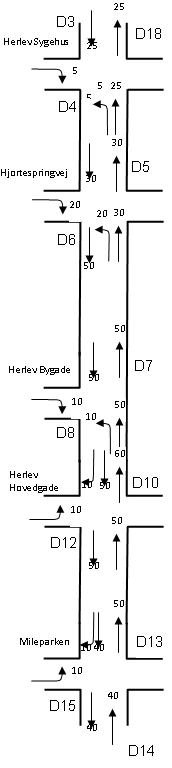
\includegraphics[scale=0.5,angle=90]{dogs_herlev.png} 
\end{center}
\caption{Layout of the partial O3 arterial in Herlev, which is under DOGS control. The arrows and numbers indicate flow direction and examples of typical vehicle count.}
\label{fig:dogs_herlev}
\end{figure}

\subsubsection*{Prediction}

DOGS is a purely traffic actuated system and no prediction is used
when the system is activated due to heavy traffic conditions.
In spite of the intended flexibility of the system this is a point
which puts high demand on the implementing traffic engineers since
traffic through the arterial must be assessed manually when the system
is put into production as well as during maintenance.

An alleviating point to the lack of prediction is the fact that the
current arterials under DOGS control are relatively small and static
predictions can be made by an experienced traffic
engineer. Furthermore, since DOGS only operate under high load
conditions, predictions become less valuable - or superfluous, even -
because all that can be said about the arterial in this case is that
it is heavily loaded with traffic.

\subsubsection*{Optimization}

Since DOGS only kicks in under congested or near-congested conditions
(for the Herlev area when the load exceeds 60\%) it is simple to
optimize the throughput since any increase in green time will just
allow more vehicles to pass (the phase is never emptied from
vehicles).

That DOGS only operates during high-congestion levels is an unusual trait for an adaptive system since they usually excel in optimization under \textit{normal} ie. uncongested load conditions (see the comparison of RHODES and a semi-actuated system in section \ref{sec:rhodes}). This can be explained from the lack of an explicitly defined objective function and optimization routine.

The objective is to keep the load degree (load/capacity) for the most heavily loaded intersection below 90\%.
To do this the common cycle time and green times are set according to the load level. The adjustments are made with a few seconds per cycle to avoid sudden, major changes in cycle time and temporary loss of coordination.

Coordination is achieved by running the signals on a common cycle time, but offsets are not adjusted when the common cycle time changes so this issue should receive further investigation.

A set of non-overlapping criteria are used to select a program with the appropiate capacity for the detected inflow. For a technical description of these criteria cf. \cite{forprojekt}

%% When naming the inflow detectors in the north- and south ends $DN$ and $DS$, respectively, the transition from pretimed control to adaptive control is decided by the constraint:
%% \begin{eqnarray*}
%% Intensity(DN) > I_{enable} & \vee & Intensity(DS) > I_{enable} \\
%% & or & \\
%% Load(DN) > L_{enable} & \vee & Load(DS) > L_{enable}
%% \end{eqnarray*}

%% For switching back to pretimed control this constraint must hold:
%% \begin{eqnarray*}
%% Intensity(DN) < I_{disable} & \wedge & Intensity(DS) < I_{disable} \\
%% & and & \\
%% Load(DN) < L_{disable} & \wedge & Load(DS) < L_{disable}
%% \end{eqnarray*}

%% To avoid hysteresis ie. constant enabling and disabling of dynamic control:
%% \begin{eqnarray}
%% I_{enable} - I_{disable} & \geq & I_{\varepsilon} \label{eqn:hysteresis_intensity} \\ 
%% L_{enable} - L_{disable} & \geq & L_{\varepsilon} \label{eqn:hysteresis_load} \\
%% I_{\varepsilon},L_{\varepsilon} & > & 0 \label{eqn:hysteresis_limits}
%% \label{eqn:hysteresis}
%% \end{eqnarray}

%% DOGS exhibits a dynamic behaviour because the permitted cycle time extensions are divided into \textit{programs} according to the intensity and load levels in the ends of the artery. These program constraints take a form which is similar to the enable- and disable constraints.

%% When deciding whether to remain in the current program, $i-1$, or switch to a program for higher demand, $i$, the following relation must be satisfied:

%% \begin{eqnarray*}
%% I_{enable,i+1} \geq & \max(Intensity(DN),Intensity(DS)) & > I_{enable,i} \\
%% & \vee & \\
%% L_{enable,i+1} \geq & \max(Load(DN),Load(DS))  & > L_{enable,i}
%% \end{eqnarray*}

%% The decision of switching from program $i$ to the program for lower demand, $i-1$, is determined by this relation:

%% \begin{eqnarray*}
%% I_{disable,i-1} \leq & \max(Intensity(DN),Intensity(DS)) & < I_{disable,i} \\
%% & \wedge & \\
%% L_{disable,i-1} \leq & \max(Load(DN),Load(DS))  & < L_{disable,i}
%% \end{eqnarray*}

%% In the DOGS controlled area in Herlev there are 8 different programs to choose from and the enable and disable thresholds for programs respect the ordering implicit in the above equations:

%% $$\lbrace I,L \rbrace_{enable,i+1} > \lbrace I,L \rbrace_{enable,i}$$
%% $$\lbrace I,L \rbrace_{disable,i-1} < \lbrace I,L \rbrace_{disable,i}$$

%% To avoid hysteresis between programs the same constraints (equations \ref{eqn:hysteresis_intensity}-\ref{eqn:hysteresis_limits}) as for switching between pretimed and dynamic control applies.

\subsubsection*{Evaluation}

Tests have shown that the system is indeed capable of increasing the
capacity, with reduced queue lengths as a result. When the arterial in
Herlev is at or above moderate load DOGS will increase the capacity by
15-25\% compared to the capacity if only the pretimed plans was in
use.


\subsection{Comparison}
The three systems presented here have different scope and as such cannot be compared directly. The RHODES system is the most general, being prepared for network wide optimization, though it will perform well along an arterial, as shown in the FHWA test case. The DOGS system is specifically designed to increase capacity along an arterial. It is very flexible but requires many input parameters, for which there is no clear selection strategy. Finally the phase-by-phase system performs advanced intersection control but has no inherent strategy for coordination, it its current state when the article was written.

Some comparisons can be made in the three main topics covered for each system ie. \textit{detection}, \textit{prediction} and \textit{optimization}.

\subsubsection*{Detection}
DOGS is the system which is most specific about detection. This is natural since it was developed by a company, which implement solutions for traffic detection, but also because it is in operation and, to the knowledge of this author, it was never simulated.

The Phase-by-Phase article has a lengthy discussion of detection technologies and placement but in fact does not make final decisions on the matter.

RHODES only mention detection to say that any technology, which can provide accurate and timely data, will suffice for prediction.

\subsubsection*{Prediction}
In this area RHODES is by far the most advanced system. The systems used at the intersection and sector level control are similar but in the detail level and scope and build on existing work. Predictions are made from detector data from upstream intersections using turning probabilities and speeds, which can be extracted from historical data.

The Phase-by-Phase system, in its current state during the writing of the article, had "perfect" prediction ie. the prediction process was directly linked to the traffic generation process of the simulator. The recommendation from Shenoda and Machemel is to further investigate the ARIMA time-series analysis framework to obtain accurate prediction for arrivals, which they argue is of dynamic nature.

DOGS has no prediction capabilities. By studying the material on the Herlev implementation and through talks with TTS and DRD it has become clear that there is a general assumption that traffic, which enters the arterial in either end is assumed to pass through the arterial. Turn-in and turn-out movements are thus expected to cancel out. This assumption could prove to be cumbersome if DOGS was to operate longer arterials with differing traffic patterns in various regions.

\subsubsection*{Optimization}
DOGS has a clear advantage in optimization since, for each cycle, the only decision to be made is whether to switch between traffic actuated control and pretimed signal plans or to change to a lower or higher capacity program. This can be done in constant time using constraints such as the one presented earlier. DOGS has no explicitly stated objective function, only a \textit{political} objective - capacity increase with reduced service for minor roads, which can be assessed in rough terms using video detectors.

Phase-by-Phase minimizes delay using tabu search by adjusting green time proportions assigned to phases. The initial solution is obtained from a proportional heuristic, using Websters results, and the 1-bit neighborhood function redistributes the green time for a single phase to the next. 
The running time of the search algorithm can be set to the maximum time before a decision must be implemented eg. until the end of the current phase.

RHODES optimization in the middle level involves generation and traversal of a conflict resolution tree in order to find the best path ie. conflict resolution according to some MOE. The optimization is made for predictions of traffic 200-300 seconds in the future. The article on RHODES does not mention how often the middle level optimization is performed, though it seems natural to reoptimize every time new predictions become available or continuously, if they are updated before the optimization completes.
The conflict resolution timing plans are fed to the intersection level optimization, which fine tunes the plans according to predicted arrival of individual vehicles using a dynamic programming approach. The optimization is valid for 45-60 seconds into the future and is rerun at the end of each phase.

\subsubsection*{Summary}
The purpose of this section was to give some in-depth reviews of systems for adaptive traffic control, which are not bound to the dense, bilevel modelling approach, which was - and still is - widely used in the litterature. 

The purpose was not to make a head-to-head comparison, in which case the RHODES system would probably prevail. The inclusion in evaluation for RT-TRACS is a testament to the completeness of RHODES and it is expected that it can easily be implemented for a real network. However, it is a complex system\footnote{This statement is backed up by the FHWA assessment of RHODES and other systems applying for RT-TRACS, see http://www.itsdocs.fhwa.dot.gov/edldocs/13480/ch3.pdf} involving many components and traffic engineers might be overwhelmed by this fact. 

DOGS has been implemented on several arterials in Denmark. It relies on the site specific knowledge of traffic engineers for definition of criteria parameters, which are most likely available, if an advanced traffic optimization system has not been employed previously. It is free from the trouble of designing sophisticated signal timing plans due to the lack of a true objective function and the fact that it only operates under medium to heavy traffic loads under which optimization reduce to the proper setting of capacity on the major road. If DOGS was to operate under off-peak traffic volumes some prediction should probably be studied and a proper objective function formulated and optimized.

The phase-by-phase system appears to have some way to go yet before becoming an option for implementation in real life intersections. Most critically is the lack of a prediction component, which, as tests show, is a determining factor for the performance of the system. 
The solution for delay calculation is the highlight of the system, especially when the phase order constraint is removed.